% Macros used only by the printed version. They must have a counterpart in macros/web.tex.
%
% This file starts with dummy macros that make the pdf compiler ignore the macros provided by
% plasTeX that only make sense for the web version.

% A Lean identifier: typewriter, breakable after each underscore (these names are long, and
% \texttt has no break points of its own, so without this they run into the margin).
\newcommand{\lname}[1]{\texttt{\renewcommand{\_}{\textunderscore\allowbreak}#1}}

% The coverage plot of the main results (plots/coverage.py), drawn at the paper's text width.
\newcommand{\coverageplot}{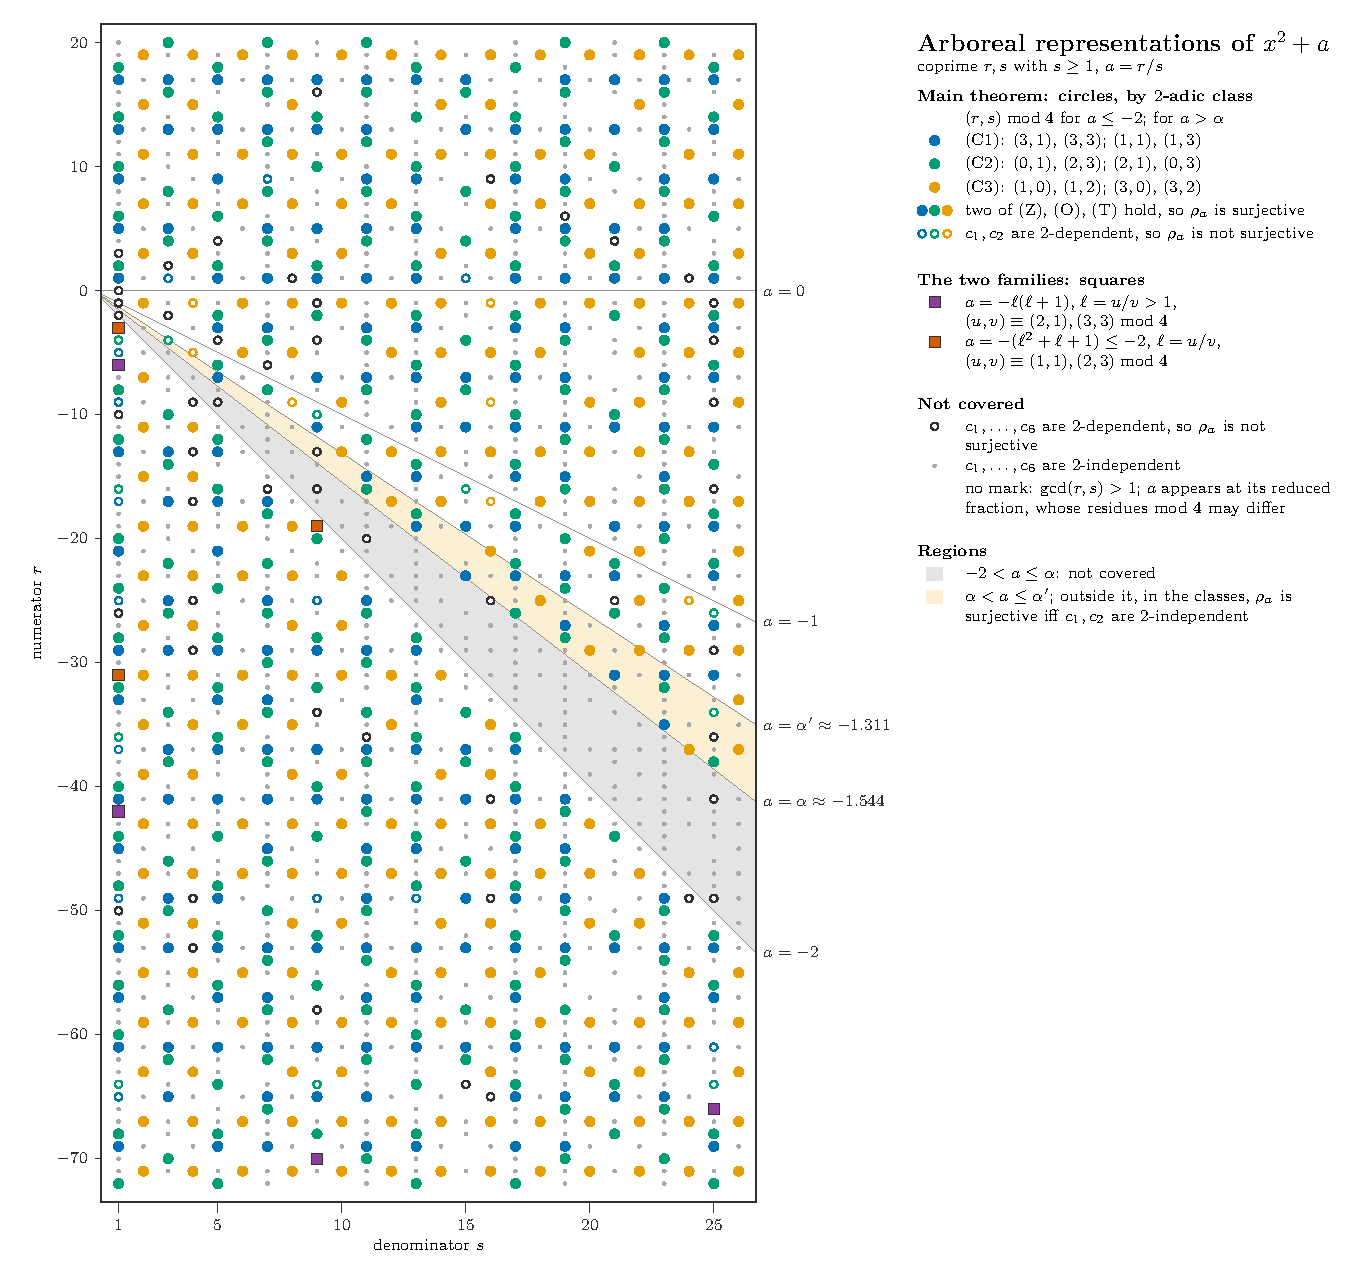
\includegraphics[width=\linewidth]{../../plots/coverage.pdf}}

% Items of a list are labelled (1), (2), ..., upright as in the paper, also when the label is
% given to \item, as in (C1). The web version does the same in templates/enumerate.jinja2s.
\setlist[enumerate,1]{label=(\arabic*)}
\setlist[enumerate]{font=\upshape}

% After \appendix, chapters are called "Appendix" and hyperref names their anchors by letters;
% Part II (\secondpart in macros/common.tex) has chapters again, with anchors of their own, and
% its longer numbers II.1, II.1.1 get wider boxes in the table of contents (tocloft).
\makeatletter
\newcommand{\restorechapters}{%
  \renewcommand{\@chapapp}{\chaptername}\renewcommand{\theHchapter}{II.\arabic{chapter}}%
  \addtocontents{toc}{\protect\setlength{\protect\cftchapnumwidth}{2.6em}%
    \protect\setlength{\protect\cftsecnumwidth}{3.4em}}}
\makeatother

\newcommand{\lean}[1]{}
\newcommand{\discussion}[1]{}
\newcommand{\leanok}{}
\newcommand{\mathlibok}{}
\newcommand{\notready}{}
% Make sure that arguments of \uses and \proves are real labels, by using invisible refs:
% latex prints a warning if the label is not defined, but nothing is shown in the pdf file.
% It uses LaTeX3 programming, this is why we use the expl3 package.
\ExplSyntaxOn
\NewDocumentCommand{\uses}{m}
 {\clist_map_inline:nn{#1}{\vphantom{\ref{##1}}}%
  \ignorespaces}
\NewDocumentCommand{\proves}{m}
 {\clist_map_inline:nn{#1}{\vphantom{\ref{##1}}}%
  \ignorespaces}
\ExplSyntaxOff
